



\section{Context/Problem Statement} \label{sec:context}
The present section introduces the synergy requirement that we aim to 
preserve while reasoning about performance requirements for access control policies and clarifies the motivation for the work presented in this paper.

\subsection{Synergy requirement related to the considered Access Control Architecture}
Most access control scenarios involve an access control policy which is modeled, analyzed and implemented as a separate component 
encapsulated in a PDP. Figure \ref{pep-pdp} illustrates the interactions between the PEPs and the PDP: the PEP calls the PDP to 
retrieve an authorization decision based on the PDP encapsulated policy. This authorization decision is made through the evaluation of rules in the policy. 
Subsequently, an authorization decision (permit/deny) is returned to the PEP.
The separation between the PEP and the PDP in access control systems simplifies policy management across many heterogeneous systems and enables to avoid
 potential risks arising from incorrect policy implementation, when the policy is hardcoded inside the business logic.

\begin{figure}[!h]
\begin{center}
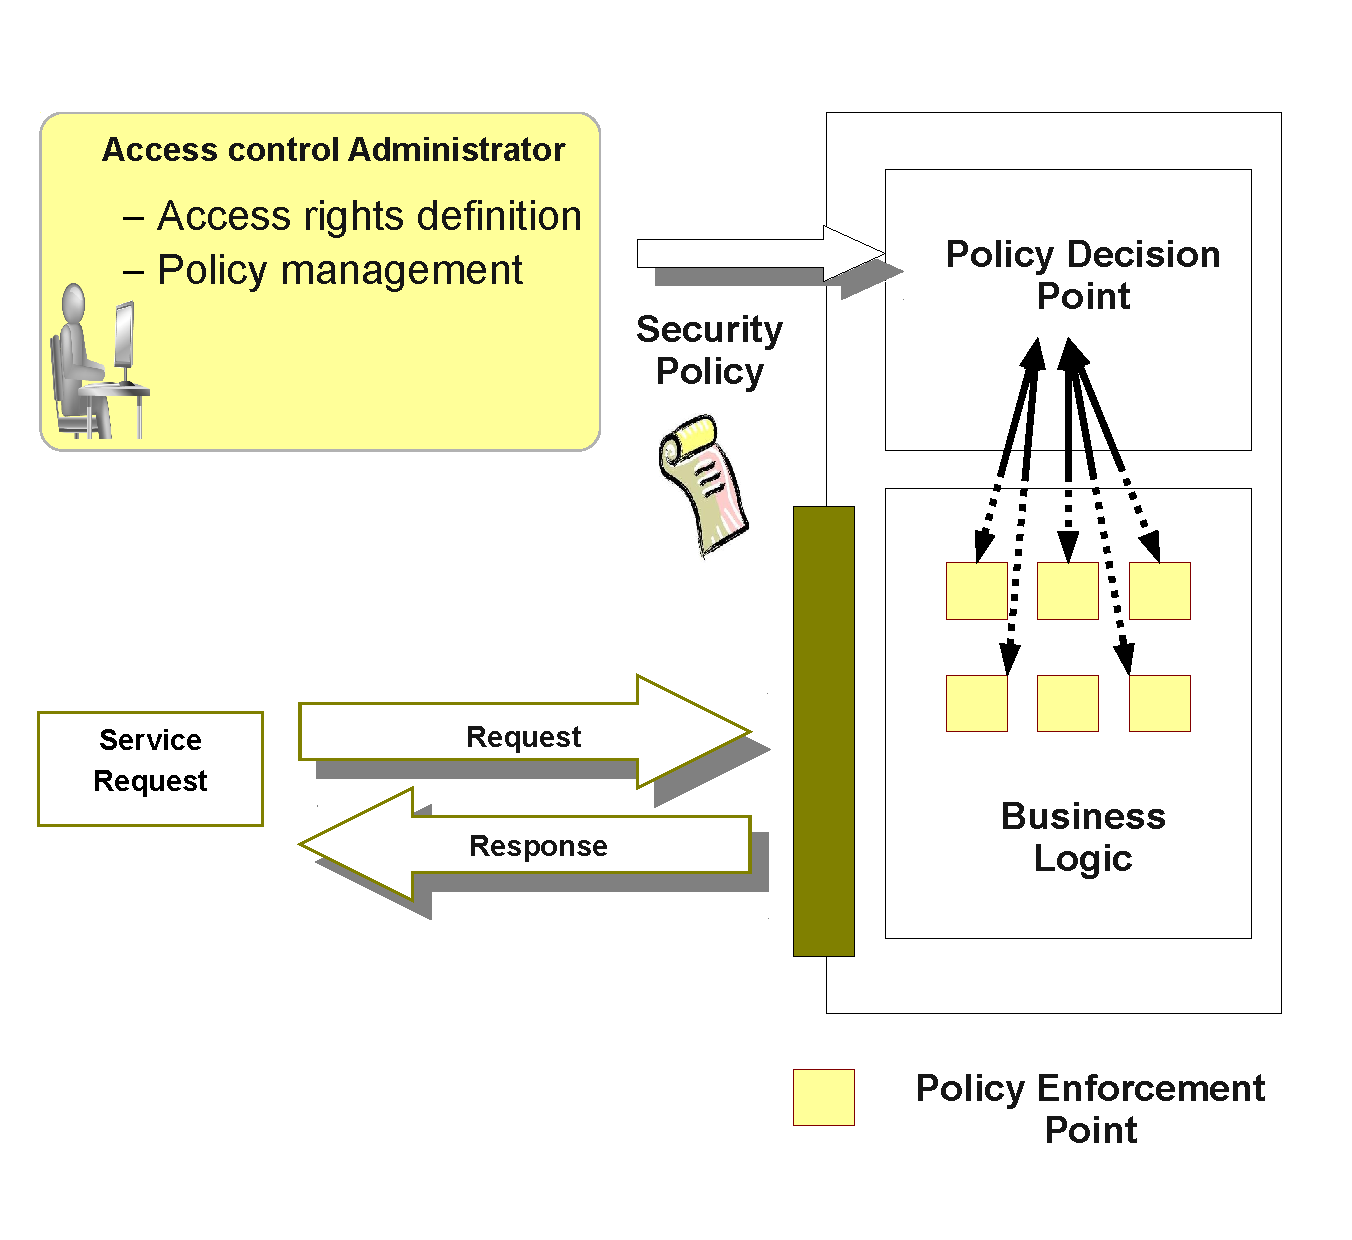
\includegraphics[width=9cm, height=8cm]{business-logic}
\caption{Access Control Request Processing}
\label{pep-pdp}
\end{center}
\end{figure}

Managing access control policies is one of the most challenging issues faced by organizations. 
Frequent changes in access control systems may be required to meet business needs. An access control system has to handle some specific 
requirements like role swap when employees are given temporary assignments, changes in the policies and procedures, 
new assets, users and job positions in the organization.
All these facts make access control architectures very difficult to manage, and plead in favor of a 
simple access control architecture that can easily handle changes in access control systems. 
Along with the reasoning about performance, we propose to maintain the simplicity of the access control architecture whose model 
is presented in Figure \ref{model}. In this model, a set of business processes, which comply to users' needs, are encapsulated in a given business logic 
which is enforced by multiple PEPs. Conceptually, the decision is decoupled from the enforcement and involves a decision making process in which each PEP 
interacts 
with one single PDP, thus a single XACML policy is evaluated to provide the suitable response for an access control request provided by a given PEP. 
\begin{figure}[!h]
\begin{center}
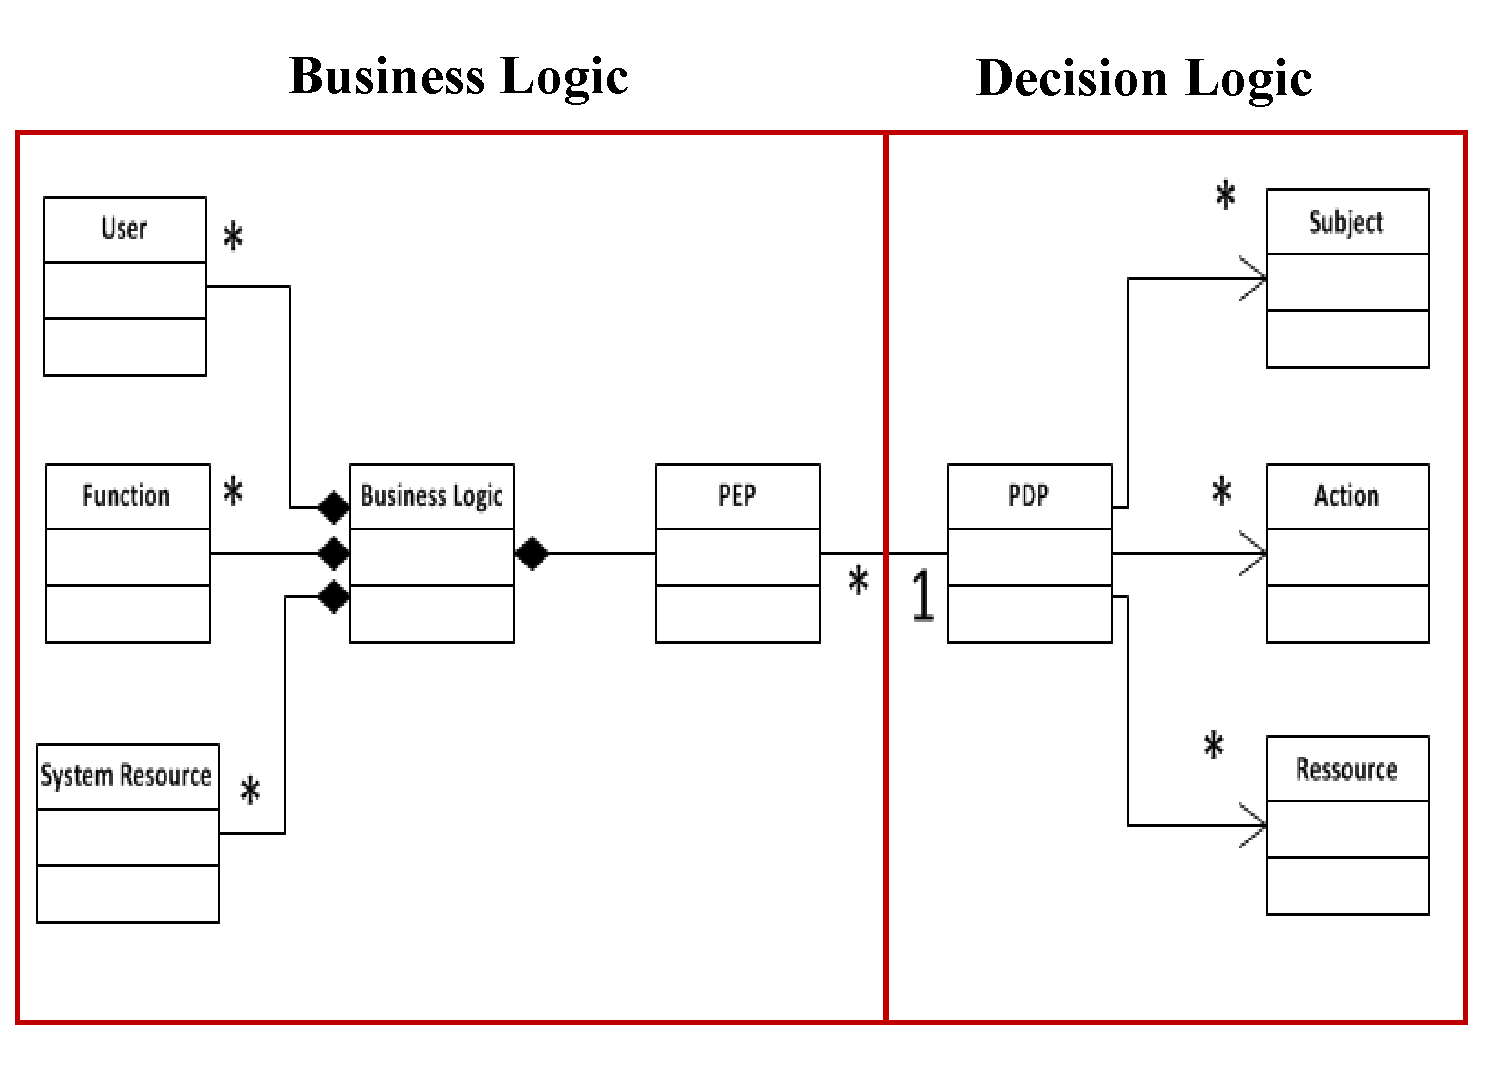
\includegraphics[height=5.5cm,width=8.5cm]{model}
\caption{The Access Control Model}
\label{model}
\end{center}
\end{figure}

Considering a single XACML policy file for each initiating PEP enables to ease policies management and to maintain a simple architecture 
in which a given PEP is mapped to a fixed PDP at each decision making process. We define the synergy requirement in the access control 
architecture by specializing access control policies to be used for a particular PEP before deployment. The goal behind maintaining a single 
policy related to each PEP in the system is to keep a strong traceability between what has been specified by the policy and the internal 
security mechanisms enforcing this policy at the business logic level. In such setting, when the access control policy rules are updated or removed, 
the related PEPs can be easily located and removed and thus the application is updated synchronously with the policy changes. 

\subsection{XACML Access Control Policies and Performance Issues}
In this paper, we focus on access control decision making for policies expressed in XACML.
XACML \cite{sunxacml} is a standard policy specification language that defines a syntax of access control policies in XML.
In the XACML paradigm, a policy set is a sequence of policies, a combining algorithm and
 a target. A policy element is expressed through a target, a set of rules and a rule combining algorithm. 
The target defines the set of resources, subjects and actions to which a rule is applicable. The rule element consists of a 
target, a condition, and an effect. The condition is a boolean expression that specifies restrictions (e.g., time and location restrictions)
 on the elements in the target. It represents 
the environmental context in which the rule applies. Finally, the effect element is either permit or deny. 
When more than one rule is applicable to a given request, the combining algorithm enables selecting which rule to choose.
For example, given two rules, which are applicable to the same request and provide different decisions,
the permit-overrides algorithm prioritizes a permit decision over the other decision.
More precisely, when using the permit-overrides algorithm, the policy evaluation engenders the following three decisions: 
\begin{itemize}
\item Permit if at least one permit rule is applicable for a request.
\item Deny if no permit rule is applicable and at least one deny rule is applicable for a request.
\item NotApplicable if no rule is applicable for a request.
\end{itemize}

Figure \ref{figur1} shows a simple XACML policy that denies subject Bob to borrow a book.
\fontsize{5}{5}
\begin{figure}[!h]
\begin{center}
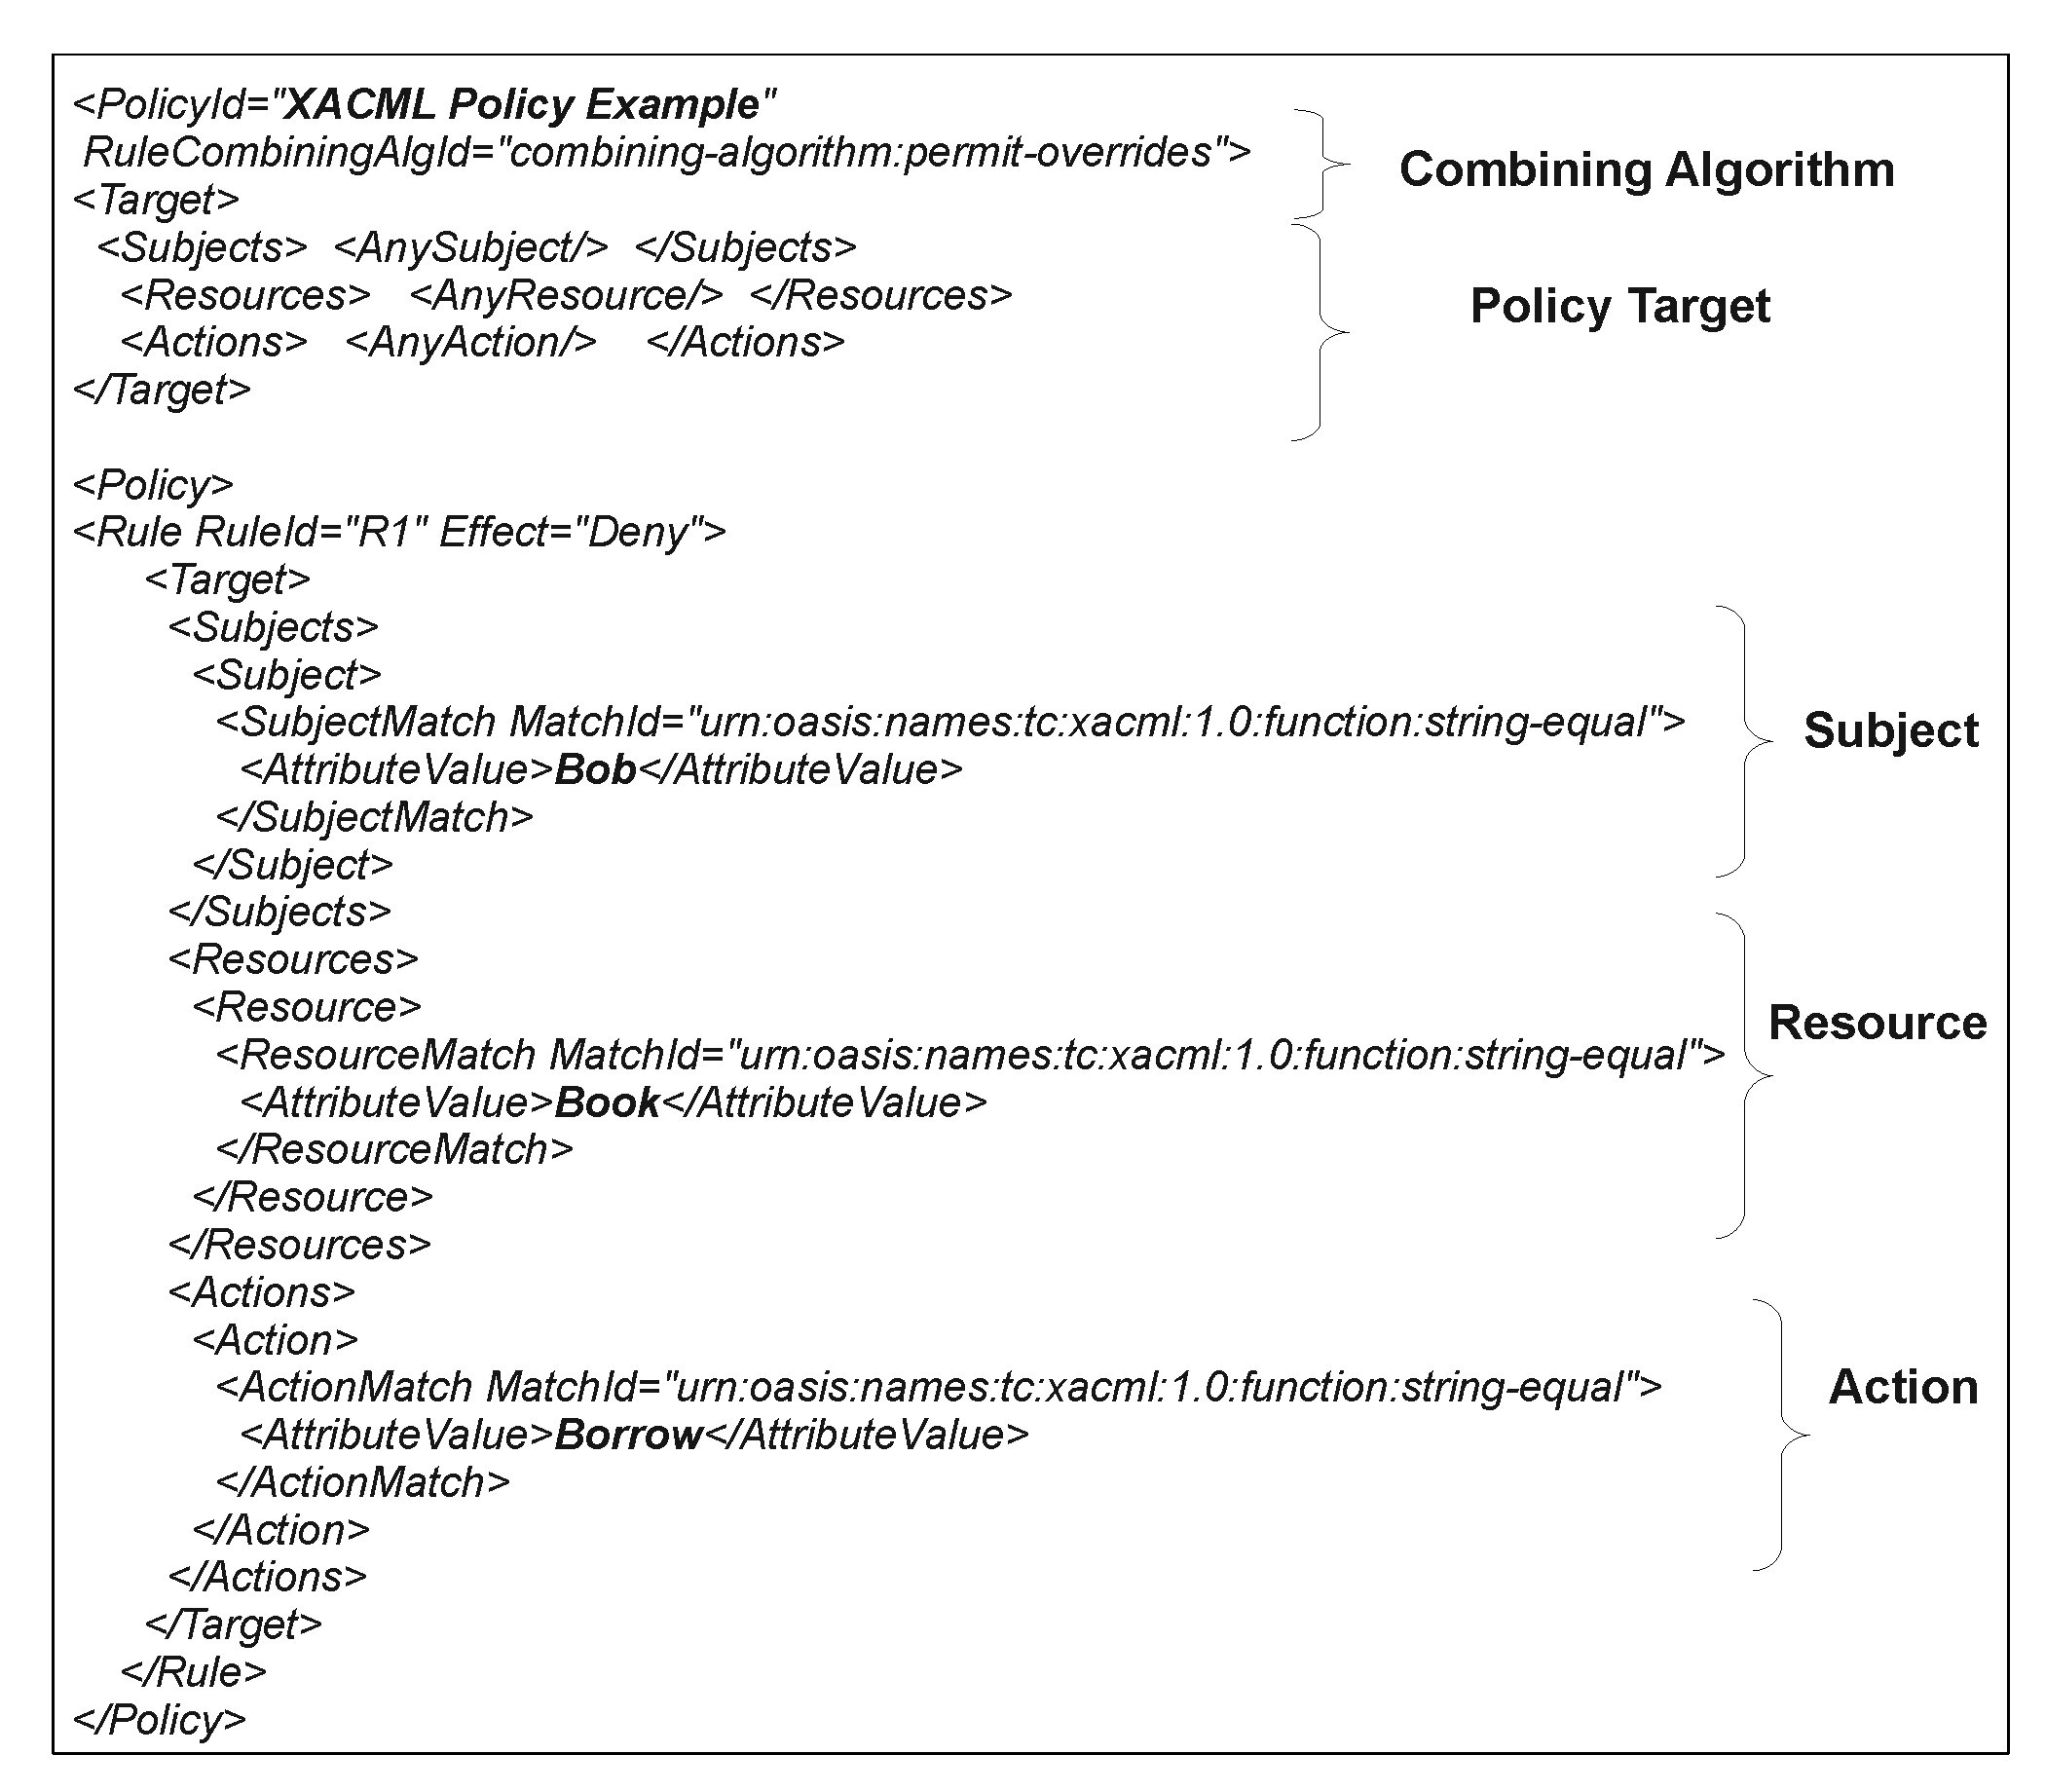
\includegraphics[width=8.6cm]{xacml}
\caption{XACML Policy Example}
\label{figur1}
\end{center}
\end{figure}

The XACML request encapsulates attributes that define which subject is requested to take an action on which protected resource in a system.
This can be under/not a condition. A request, which satisfies both target and condition in a rule, is evaluated
to decision specified in the rule's effect element. If the request does not satisfy target and condition elements in any rule, its response yields ``NotApplicable'' decision.
\\XACML enables administrators to externalize access control policies for the sake of interoperability since access control policies can be designed 
independently from the underlying programming language or platform. Such flexibility enables to easily update the access control policy to support new requirements.
%\centering
%\figure[DREF metamodel\label{fig:drefMM}]
%        {\includegraphics[width=0.5\textwidth]{figure/drefMM}}
%\figure[SETER Process: Security Testing for Resilient Systems 
%\label{fig:seter}] {\includegraphics[width=0.49\textwidth]{figure/seter}}
%\caption{DREF and SETER: Conceptual and Operational Frameworks for evaluating resilient systems}
%\end{figure*}

However, the increasing complexity of organizations in terms of structure, relationships, activities, and access control requirements has impacted 
access control policy design. This has led to deal with access control policies where the number of rules depicting the associations between resources, 
users and actions is in continuous increase. Moreover, the policy is usually centralized in a single point PDP, which has to manage 
multiple access control requests. These observations raise performance concerns related to request evaluation time for XACML access control policies and may 
degrade the system efficiency and slow down the overall business processes. 
Moreover, considering XACML specifities, some factors may lead to degrade XACML requests evaluation performance: 

\begin{itemize}
\item An XACML policy may contain several attributes that constitute descriptive information about the target elements, the retrieval of
 varying size of attributes values for each request within XML elements in a request, may increase the evaluation time.
\item A PolicySet includes a set of policies, the effect of the whole PolicySet is determined by combining the effects of 
the policies according to a combining algorithm, the computation of resulting effect from policies is also considered as a potential evaluation
 time latency.
\item Conditions evaluation in XACML rules may slow down the decision making process since these conditions can be complex because they can 
be built from an arbitrary nesting of non-boolean functions and attributes. 
\end{itemize}

